\documentclass[../notes.tex]{subfiles}

\pagestyle{main}
\renewcommand{\chaptermark}[1]{\markboth{\chaptername\ \thechapter\ (#1)}{}}
\setcounter{chapter}{6}

\begin{document}




\chapter{Electronic Relaxation}
\section{Office Hours (Moe)}
\begin{itemize}
    \item \marginnote{2/13:}Use chemical shift as your $x$-axis in NMR plots.
    \item Hexylamine is our substance.
    \item Interpreting NMR data files: Column E is chemical shift; column C is peak intensity. Column D is hertz (not chemical shift).
    \begin{itemize}
        \item Chemical shift is in the rightmost column.
    \end{itemize}
    \item Fitting tutorial: If solver still isn't helping (you get an error message and no convergence), divide the absolute intensities by a million. You can also do this from the get-go.
    \item $M_z$ should be calculated for each carbon; it is the absolute integral value in the all-integrals spreadsheet.
    \item Don't let the peaks overlap in the plot of multiple vertically offset $T_1$ values.
    \begin{itemize}
        \item Use 3 plots.
    \end{itemize}
    \item R outputs standard error values automatically.
    \begin{itemize}
        \item In Excel, it's much more difficult.
        \item A residuals plot is a good thing to include, but there won't be points for it. Standard error also isn't worth points. Sarah will have them upload the rubric. Sarah opened the door to email her.
        \item We need standard error for all 6 regressions.
    \end{itemize}
    \item Sarah will send a source for literature values.
\end{itemize}



\section{Lecture 12: Electronic Relaxation and Fluorescence Spectroscopy}
\begin{itemize}
    \item \marginnote{2/14:}Today: What happens after absorption (fluorescence and relaxation).
    \item Motivating question: What is the fate of electronic excitations?
    \begin{itemize}
        \item Absorption to an electronic excited state takes a lot of energy.
        \item This energy needs to be dissipated to return to equilibrium via
        \begin{equation*}
            \ce{A^* -> A + energy}
        \end{equation*}
        \item Many possible routes (radiative [releasing low-energy photons] and non-radiative [various]).
    \end{itemize}
    \item Review: Electronic absorption leads to vibrational excitation which relaxes vibrationally.
    \begin{figure}[H]
        \centering
        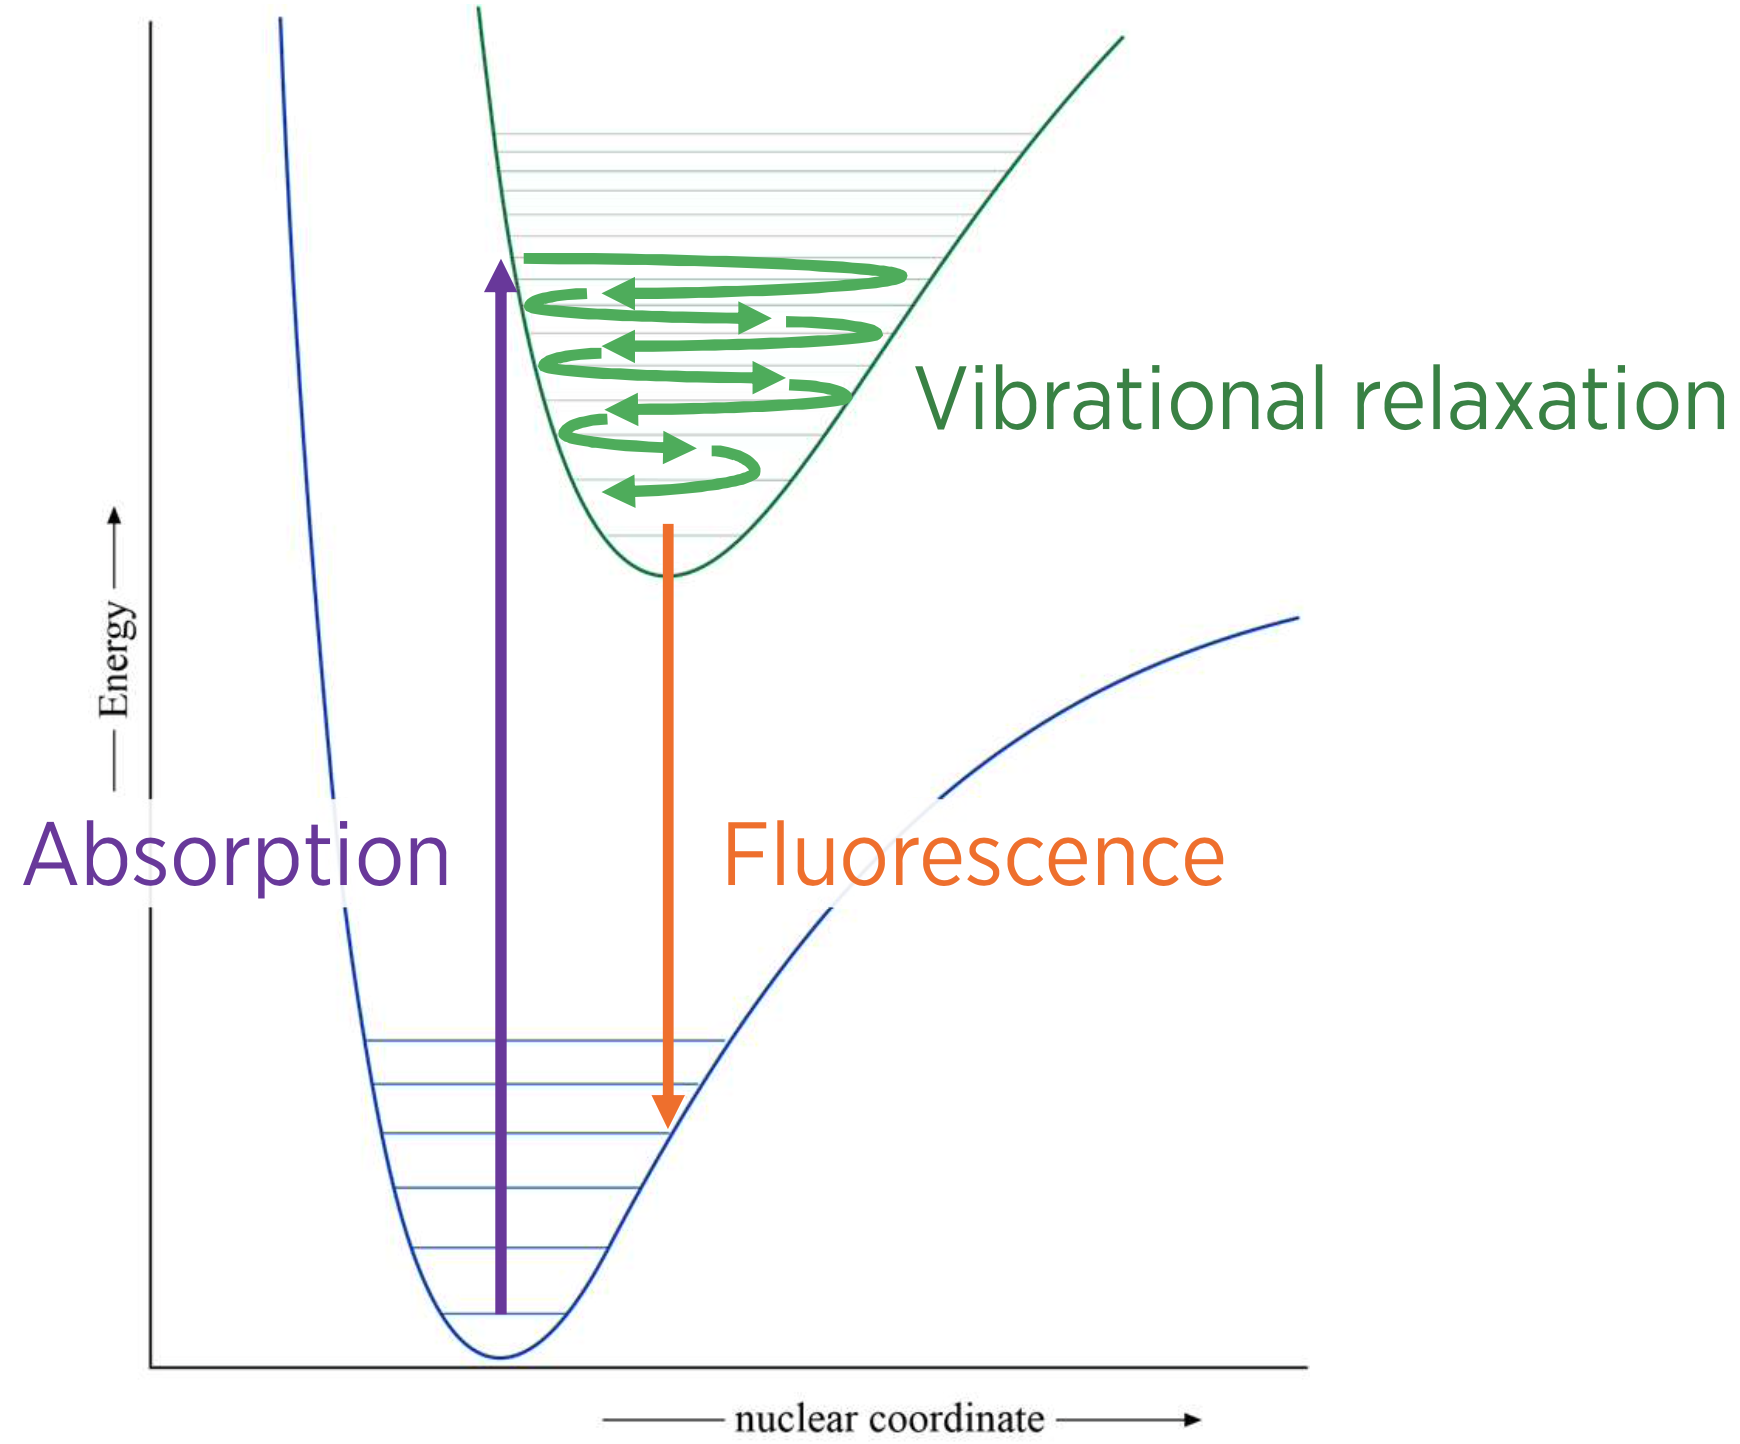
\includegraphics[width=0.4\linewidth]{excitationSteps.png}
        \caption{The photophysical excitation process.}
        \label{fig:excitationSteps}
    \end{figure}
    \begin{itemize}
        \item Vibrational energy dissipates non-radiatively via intramolecular vibrational energy redistribution and intermolecular collisions.
        \begin{itemize}
            \item No change in electronic state is involved.
        \end{itemize}
        \item The radiative path (fluorescence) is slower.
        \begin{itemize}
            \item $k_\text{rad}\ll k_\text{IVR}$.
            \item Most fluorescence occurs from $v'=0$. Further relaxation requires a change of electronic state.
        \end{itemize}
        \item Time scale of relevant processes.
        \begin{itemize}
            \item The vibrational period of a molecule is \SIrange{10}{100}{\femto\second}.
            \item Vibrational relaxation in solution takes \SIrange{1}{10}{\pico\second}.
            \item Fluorescence emission takes \SIrange{1}{10}{\nano\second}.
        \end{itemize}
        \item Once you get into the ground state, you have further vibrational relaxation.
    \end{itemize}
    \item $\bm{k_\textbf{rad}}$: The radiative fluorescence emission rate.
    \item $\bm{k_\textbf{nr}}$: The rate of all nonradiative processes leaving the flourescent state. \emph{Given by}
    \begin{equation*}
        k_\text{nr} = \sum_ik_{\text{nr},i}
    \end{equation*}
    \item $\bm{k_\textbf{IVR}}$: The \underline{i}ntramolecular \underline{v}ibrational \underline{r}elaxation rate.
    \item \textbf{Reorganization energy}: The amount of energy dissipated on one of the potential energy surfaces. \emph{Denoted by} $\lambda$.
    \begin{figure}[H]
        \centering
        \begin{subfigure}[b]{0.35\linewidth}
            \centering
            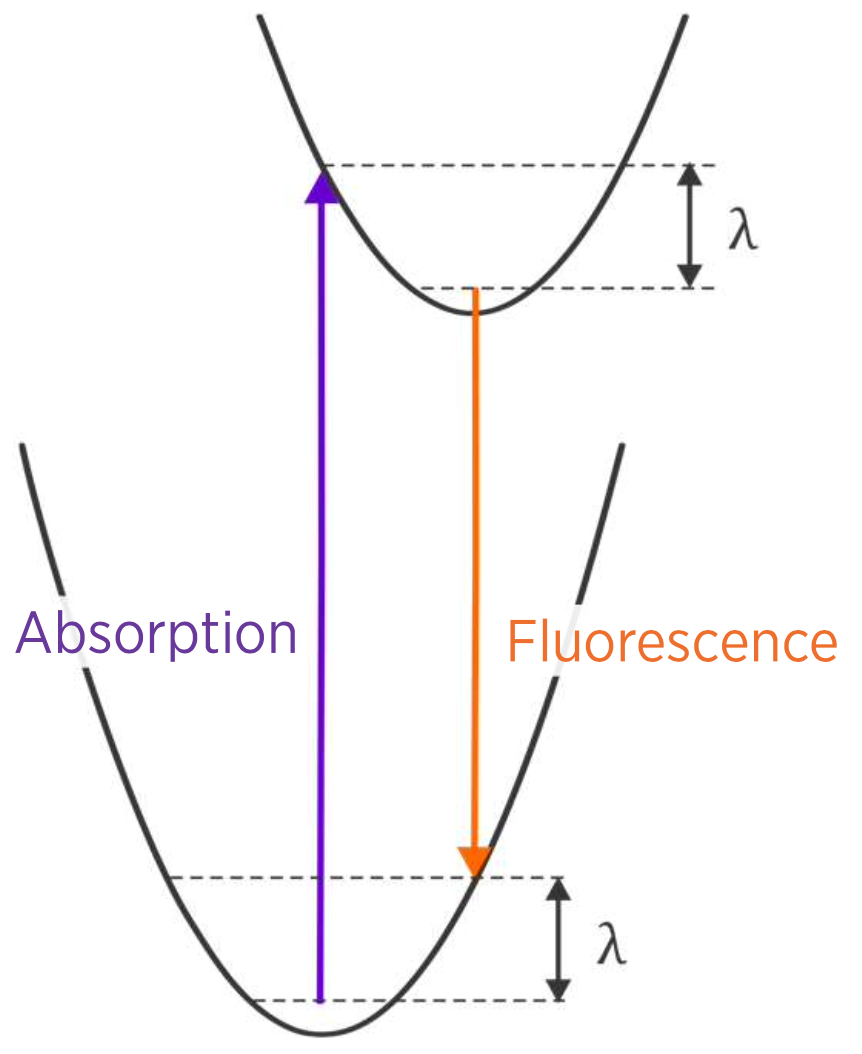
\includegraphics[width=0.6\linewidth]{reorgEa.png}
            \caption{Reorganization energy.}
            \label{fig:reorgEa}
        \end{subfigure}
        \begin{subfigure}[b]{0.35\linewidth}
            \centering
            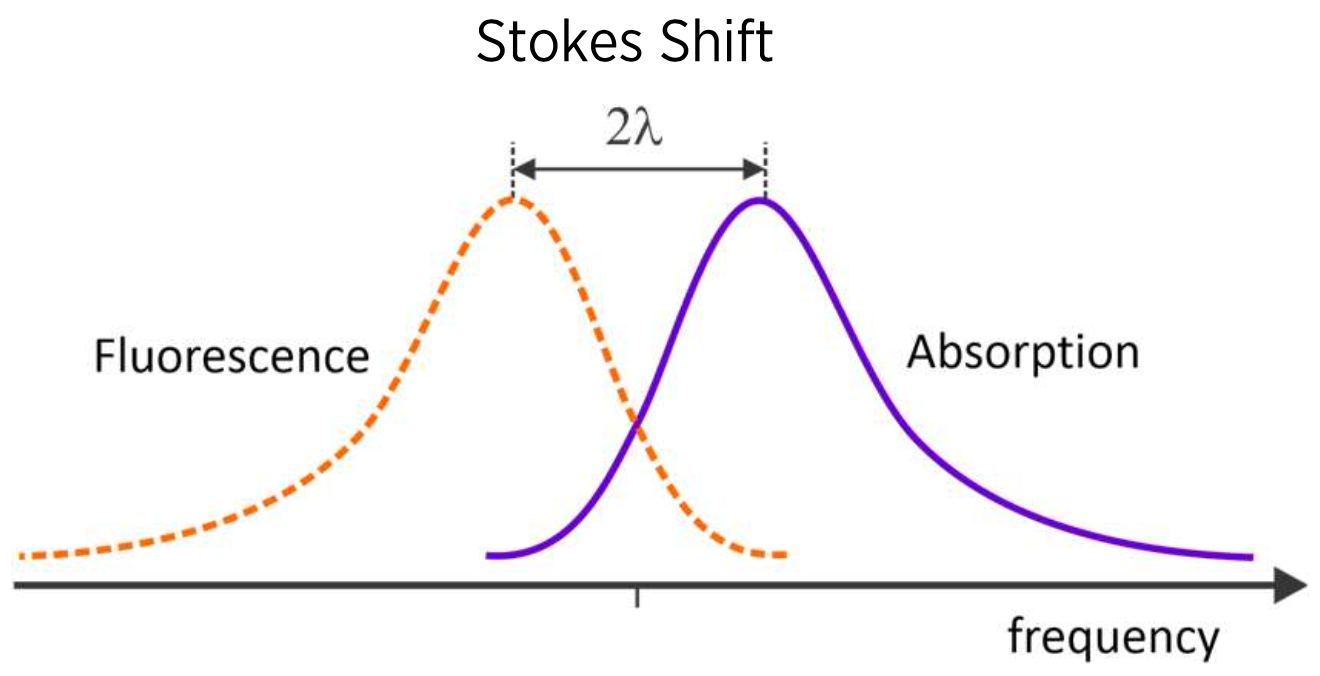
\includegraphics[width=0.95\linewidth]{reorgEb.png}
            \caption{Stokes shift.}
            \label{fig:reorgEb}
        \end{subfigure}
        \caption{Quantifying photophysical reorganization.}
        \label{fig:reorgE}
    \end{figure}
    \begin{itemize}
        \item Per the above, some energy is dissipated in both the ground and excited states. The amount dissipated in both is (roughly??) the same and is denoted by $\lambda$.
        \item The overall energy shift is known as the \textbf{Stokes shift} and is the sum of the two reorganizational energies.
    \end{itemize}
    \item \textbf{Stokes shift}: The difference in energy absorbed vs. energy fluoresced. \emph{Denoted by} $\bm{2\lambda}$.
    \item Other non-radiative intramolecular electronic relaxation process.
    \item Internal conversion.
    \begin{figure}[h!]
        \centering
        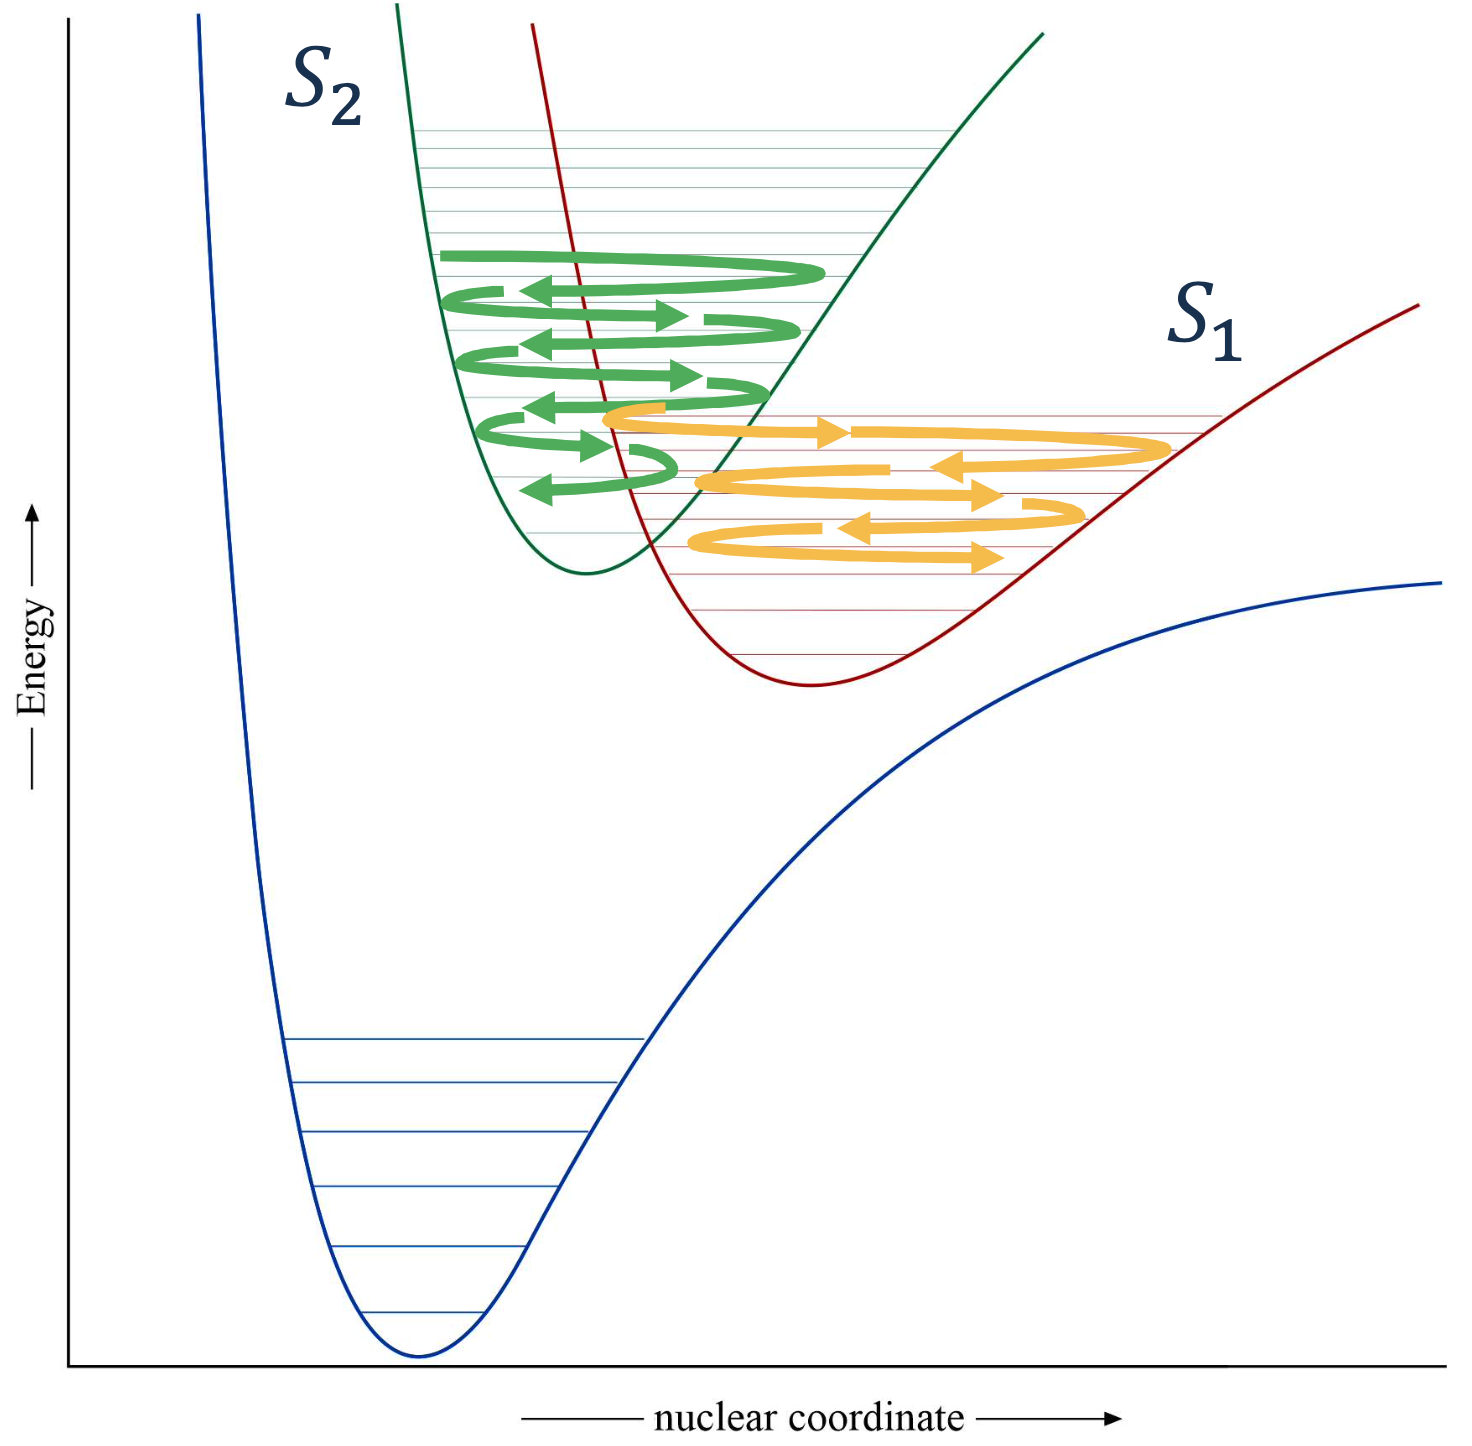
\includegraphics[width=0.3\linewidth]{internalConversion.png}
        \caption{Internal conversion.}
        \label{fig:internalConversion}
    \end{figure}
    \begin{itemize}
        \item Essentially, exchange between higher lying excited singlet states can be very efficient.
        \item We obey the \textbf{energy gap law}.
    \end{itemize}
    \item \textbf{Energy gap law}: The non-radiative relaxation rate scales exponentially in the energy gap between the initial and final states. \emph{Given by}
    \begin{equation*}
        k_\text{nr} \propto \exp(-\Delta E)
    \end{equation*}
    \item Intersystem crossing.
    \begin{itemize}
        \item Non-radiative singlet to triplet energy transfer.
        \item We have to consider what happens when we change the spin angular momentum. Because this takes energy, this is quite improbable unless we have something like spin-orbit coupling present.
        \item Nominally forbidden in closed shell molecules. Hence, it is slow.
        \begin{itemize}
            \item $ms$ in closed shell organics.
            \item $ps$-$ns$ in metal coordination compounds via SOC, MLCT.
        \end{itemize}
    \end{itemize}
    \item \textbf{Phosphorescence}: Luminescence from triplet states.
    \begin{itemize}
        \item Occurs on a very slow microsecond to millisecond time scale.
    \end{itemize}
    \item Intermolecular processes.
    \begin{figure}[h!]
        \centering
        \begin{subfigure}[b]{0.24\linewidth}
            \centering
            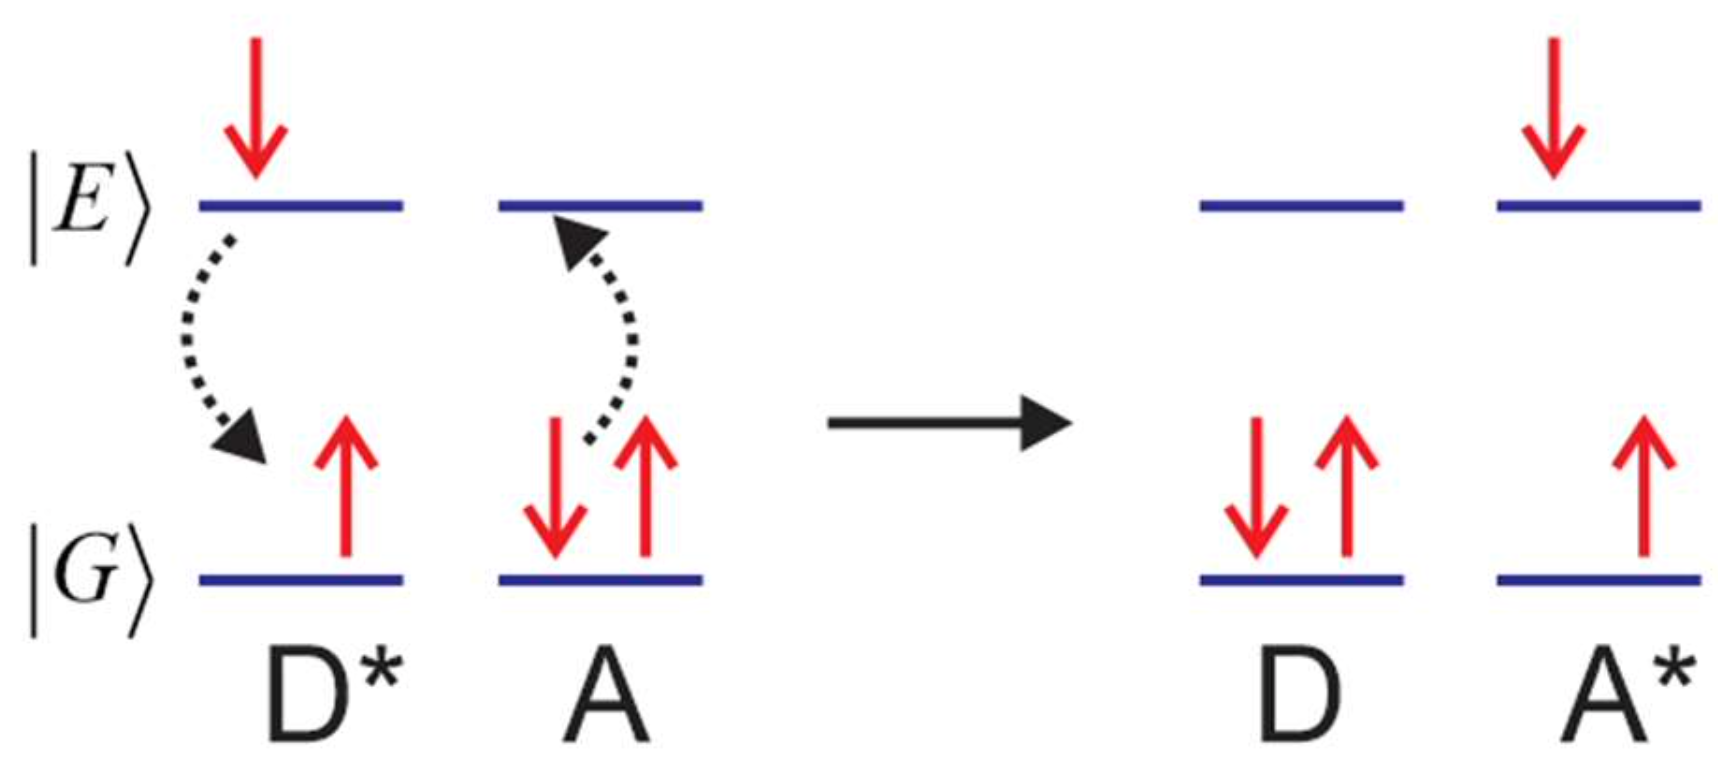
\includegraphics[width=0.8\linewidth]{interRelaxa.png}
            \caption{Forster ET.}
            \label{fig:interRelaxa}
        \end{subfigure}
        \begin{subfigure}[b]{0.24\linewidth}
            \centering
            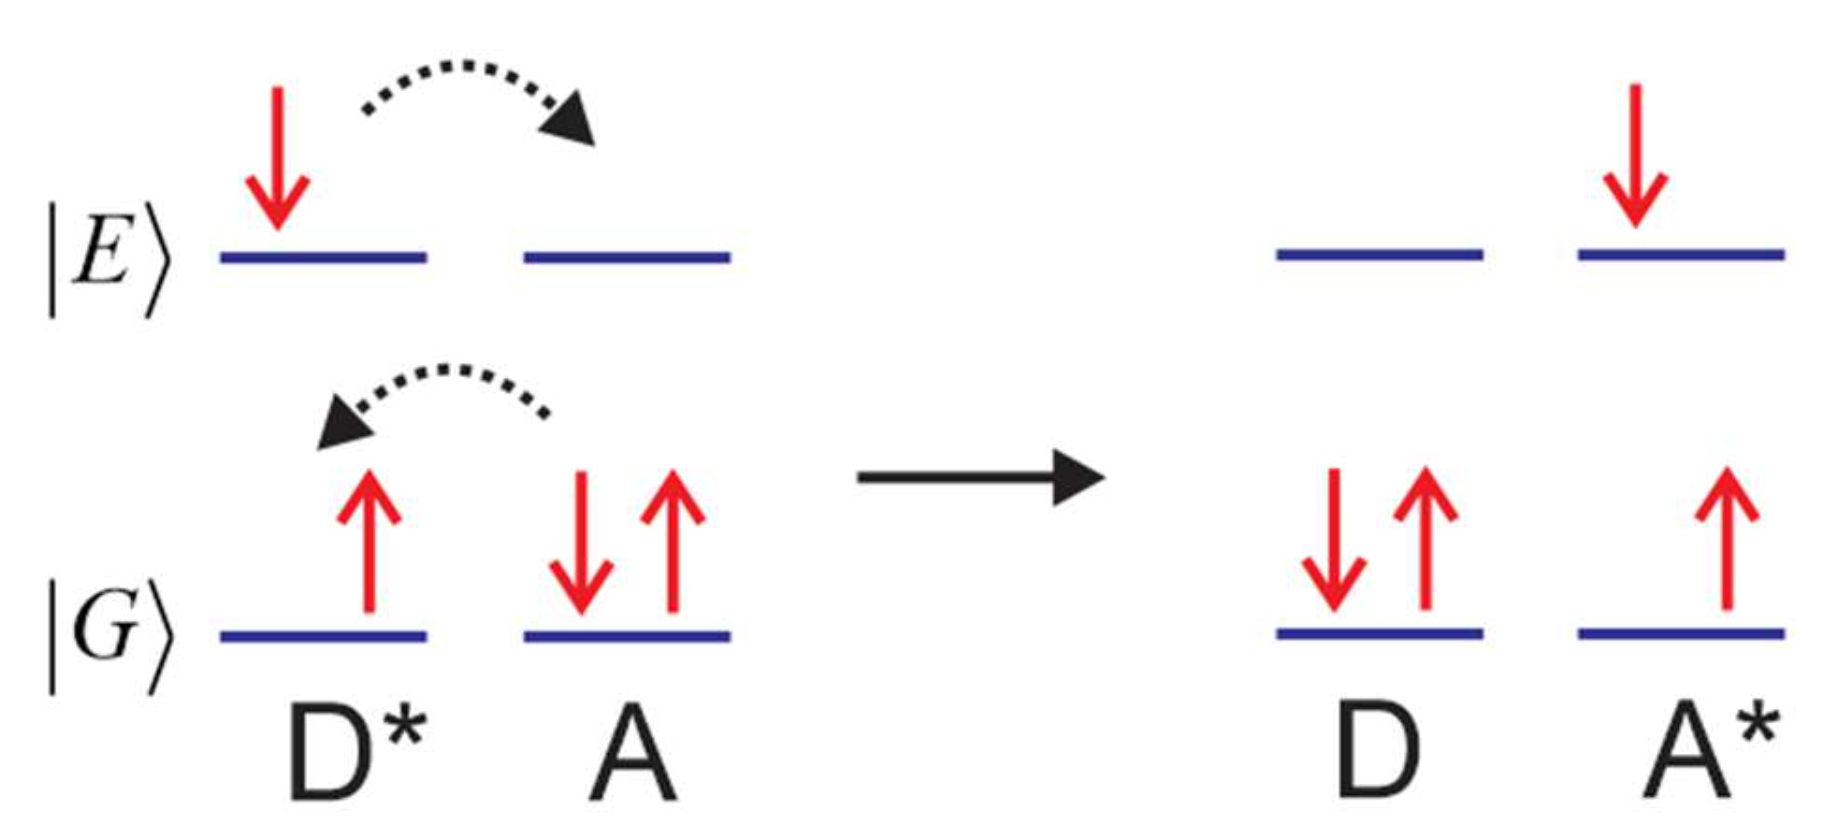
\includegraphics[width=0.8\linewidth]{interRelaxb.png}
            \caption{Dexter ET.}
            \label{fig:interRelaxb}
        \end{subfigure}
        \begin{subfigure}[b]{0.24\linewidth}
            \centering
            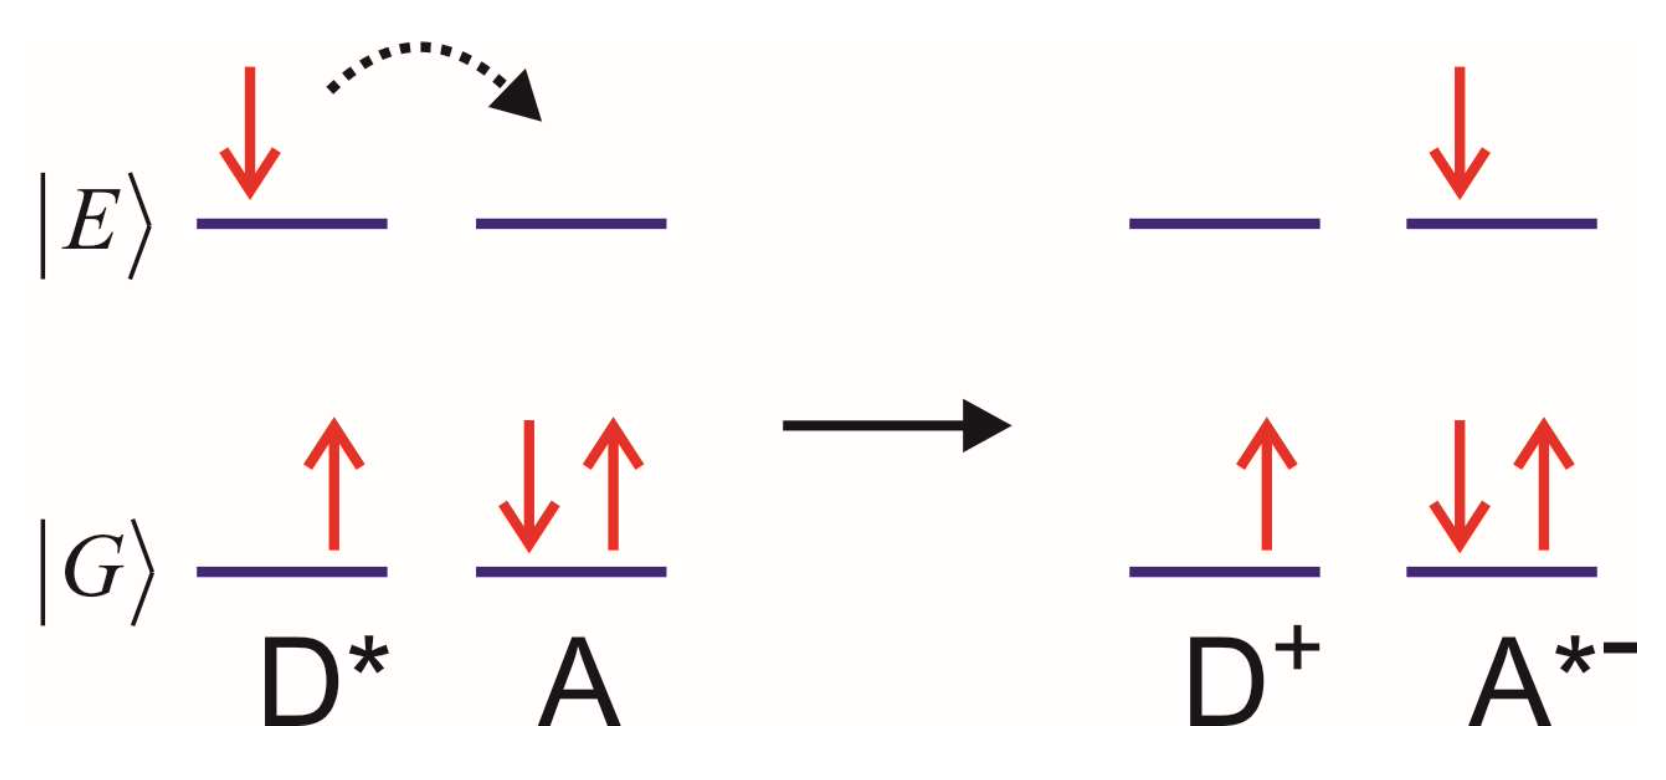
\includegraphics[width=0.8\linewidth]{interRelaxc.png}
            \caption{MLCT.}
            \label{fig:interRelaxc}
        \end{subfigure}
        \begin{subfigure}[b]{0.24\linewidth}
            \centering
            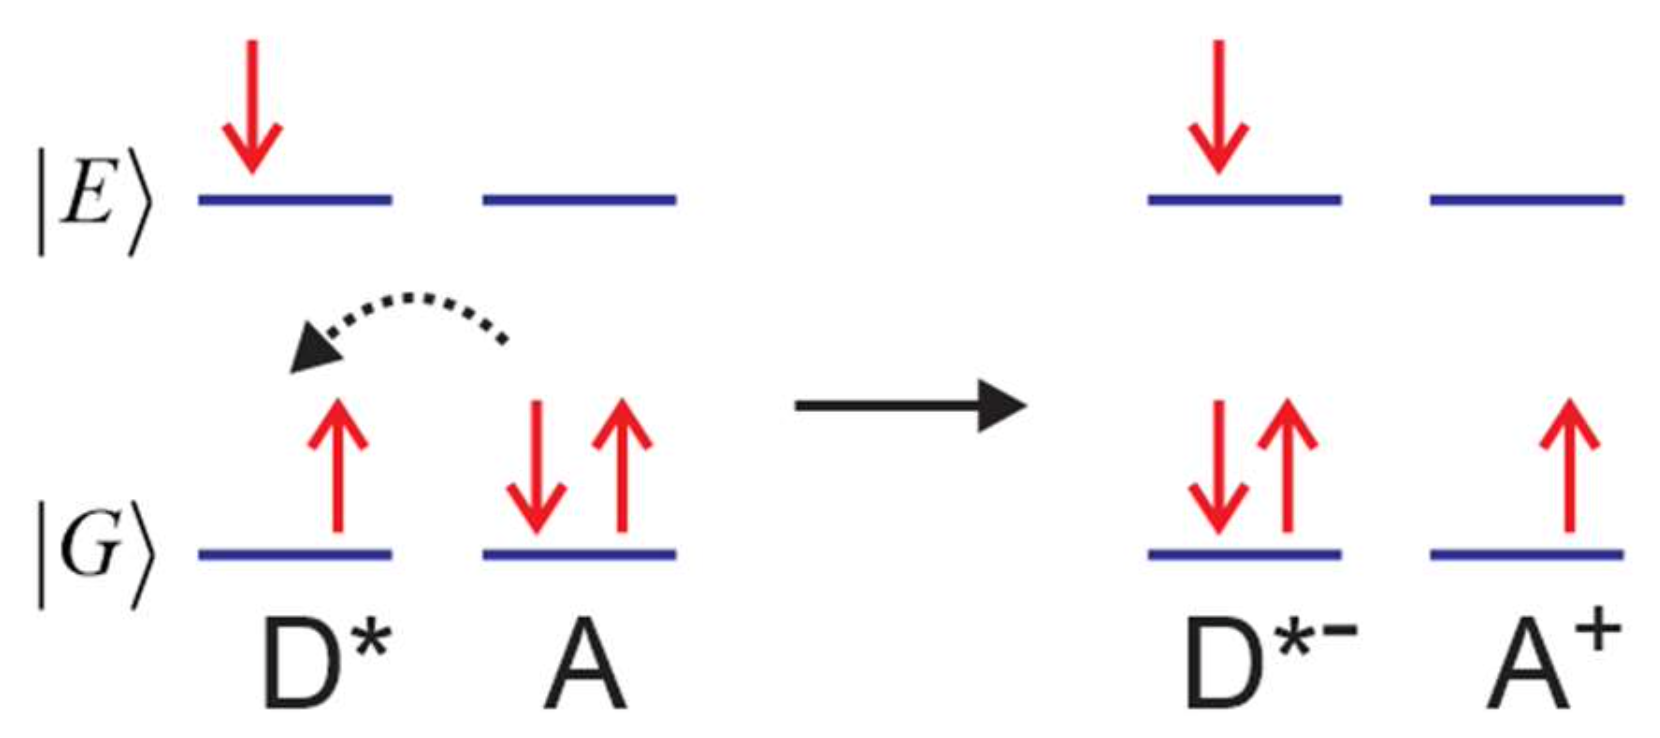
\includegraphics[width=0.8\linewidth]{interRelaxd.png}
            \caption{LMCT.}
            \label{fig:interRelaxd}
        \end{subfigure}
        \caption{Intermolecular relaxation mechanisms.}
        \label{fig:interRelax}
    \end{figure}
    \begin{itemize}
        \item Forster energy transfer (through space), aka, electronic resonance energy transfer.
        \begin{itemize}
            \item Two dipoles couple, and one drives the other.
        \end{itemize}
        \item Dexter energy transfer.
        \begin{itemize}
            \item Wavefunction overlap and electrons move.
        \end{itemize}
        \item MLCT (electron transfer).
        \begin{itemize}
            \item Donor gives a high energy electron to an acceptor.
        \end{itemize}
        \item LMCT (hole transfer).
        \begin{itemize}
            \item Donor gives a hole to the acceptor.
            \item Electronic excitation brings electron density to the metal center.
        \end{itemize}
    \end{itemize}
    \item Triplet quenching by oxygen.
    \begin{figure}[h!]
        \centering
        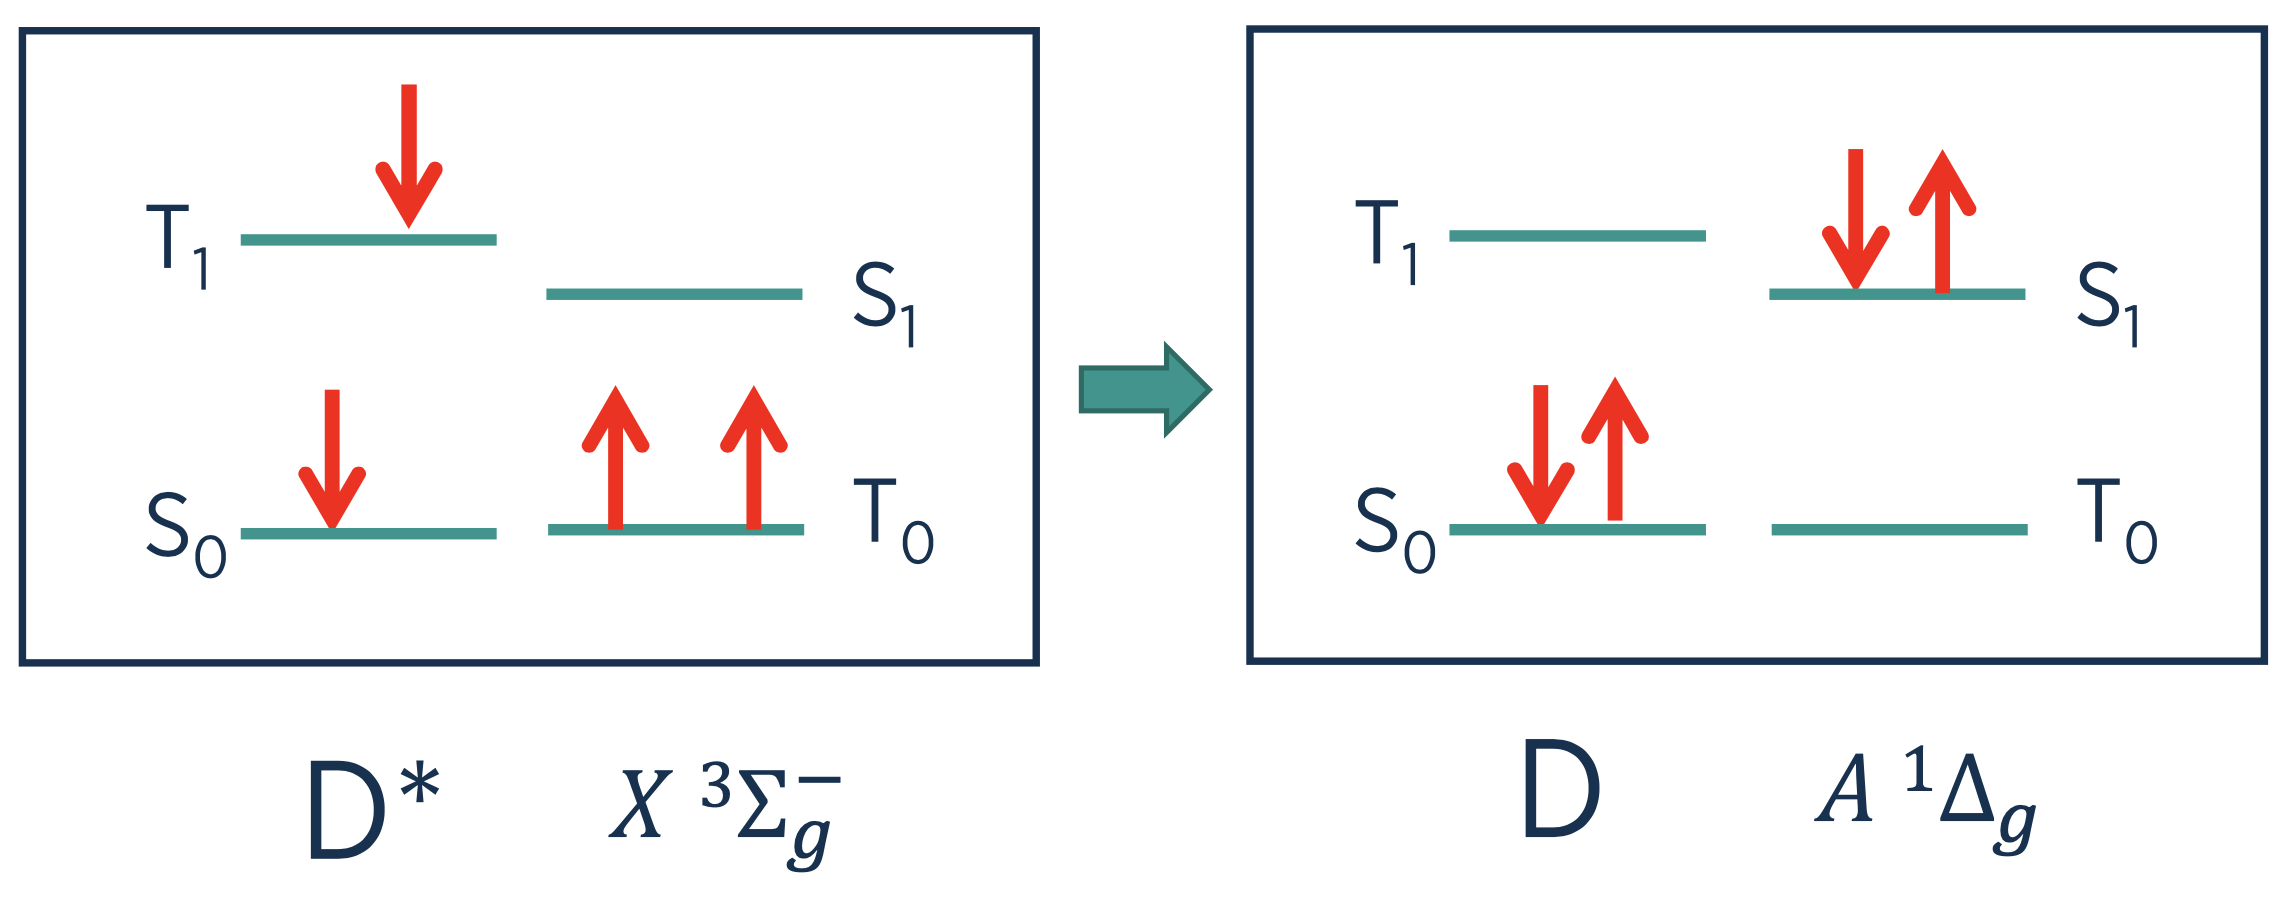
\includegraphics[width=0.4\linewidth]{O2TripQuench.png}
        \caption{Triplet quenching by oxygen.}
        \label{fig:O2TripQuench}
    \end{figure}
    \begin{itemize}
        \item Oxygen is a rare ground-state triplet compound.
        \item Thus, it can easily transfer electron density to other excited triplets, quenching them.
        \item Rate is partially determined by the proximity of oxygen to whatever it's quenching.
    \end{itemize}
    \item Photochemistry summary.
    \begin{itemize}
        \item Light provides energy to surmount activation barriers (relevant to atmospheric chemistry, photosynthesis).
        \item Photodissociation (relevant to bond cleavage, ligand release, photoacids, photoionization, and radicals).
        \item Electron transfer and proton-coupled electron transfer.
        \item Photoisomerization (see below).
    \end{itemize}
    \item Photoisomerization.
    \begin{figure}[h!]
        \centering
        \begin{subfigure}[b]{0.5\linewidth}
            \centering
            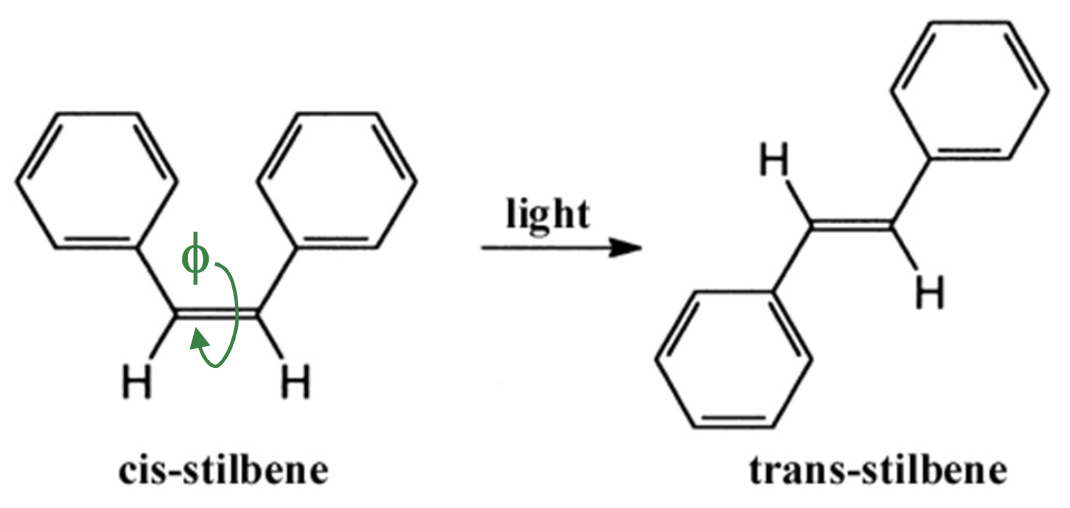
\includegraphics[width=0.8\linewidth]{photoisomerizationa.png}
            \caption{Example reaction.}
            \label{fig:photoisomerizationa}
        \end{subfigure}
        \begin{subfigure}[b]{0.3\linewidth}
            \centering
            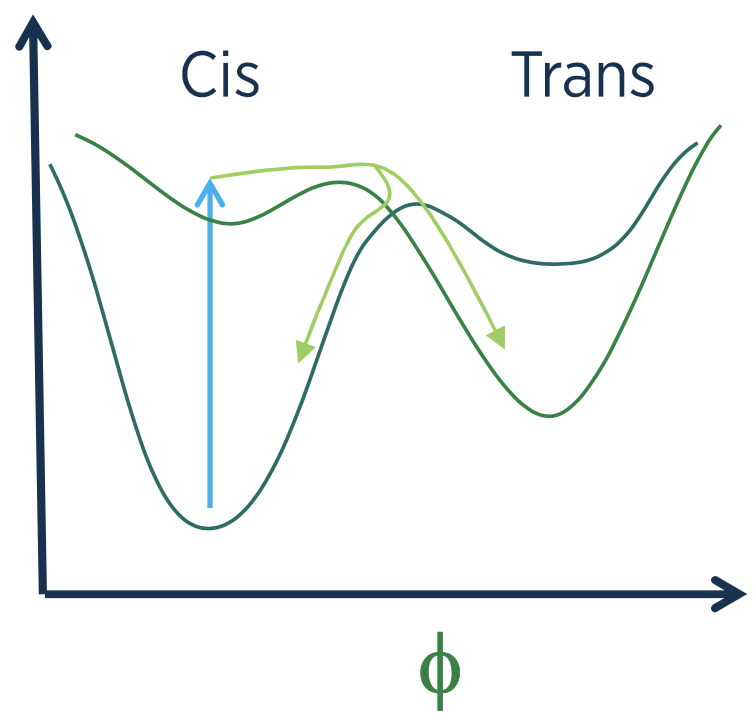
\includegraphics[width=0.8\linewidth]{photoisomerizationb.png}
            \caption{Mechanism.}
            \label{fig:photoisomerizationb}
        \end{subfigure}
        \caption{Photoisomerization.}
        \label{fig:photoisomerization}
    \end{figure}
    \begin{itemize}
        \item Stilbene possesses \emph{cis}/\emph{trans} photoisomerization.
    \end{itemize}
    \item Quantities in fluorescence spectroscopy.
    \item \textbf{Fluorescence quantum yield}: The probability that an absorbed photon led to emission of a photon via fluorescence. \emph{Denoted by} $\bm{\Phi}$. \emph{Given by}
    \begin{equation*}
        \Phi = \frac{\text{\# of fluorescence photons emitted}}{\text{\# of input photons absorbed}}
        = \frac{k_\text{rad}}{k_\text{rad}+k_\text{nr}}
    \end{equation*}
    \begin{itemize}
        \item Tells you how good of a fluorophore your molecule is, i.e., how good it is at absorbing light and turning it back into fluorescence.
    \end{itemize}
    \item $\bm{k_\textbf{f}}$: The rate constant for fluorescence emission. \emph{Given by}
    \begin{equation*}
        k_\text{f} = k_\text{rad}+k_\text{nr}
    \end{equation*}
    \item \textbf{Fluorescence lifetime}: The time constant relating to the rate of fluorescence emission. \emph{Denoted by} $\bm{\tau}$. \emph{Given by}
    \begin{equation*}
        \tau = \frac{1}{k_\text{f}}
    \end{equation*}
    \item The underlying theory behind the fluorescence lifetime.
    \begin{itemize}
        \item The measured fluorescence intensity $I(t)$ is proportional to the number of excited states, i.e.,
        \begin{equation*}
            I(t) \propto \ce{A^*}(t)
        \end{equation*}
        \item The rate law for fluorescence decay is
        \begin{align*}
            \dv{\ce{A^*}}{t} &= -k_\text{f}\ce{A^*}\\
            I(t) &= I(0)\exp(-k_\text{f}t)
        \end{align*}
    \end{itemize}
    \item Implication: We can use fluorescence to probe non-radiative processes.
    \item Example: Quenching experiments.
    \begin{itemize}
        \item Object of study: Short-range interactions that lead to rapid non-radiative relaxation.
        \item Background: The fluorescence lifetime in the absence of quencher is $\tau_0=k_0^{-1}$. The quencher results in an additional route for non-radiative relaxation.
        \begin{itemize}
            \item Implication: The fluorescence lifetime $\tau$ decreases: $\tau<\tau_0$.
            \item If $[\ce{Q}]$ denotes the concentration of the quencher and $k_q$ denotes the rate constant associated with quenching by the quencher, then we have
            \begin{align*}
                -\dv{\ce{A^*}}{t} &= k_0\ce{A^*}+k_q\ce{A^*}[\ce{Q}]\\
                &= (k_0+k_q[\ce{Q}])\ce{A^*}
            \end{align*}
            so that
            \begin{equation*}
                \frac{1}{\tau} = k_0+k_q[\ce{Q}]
                = \frac{1}{\tau_0}+k_q[\ce{Q}]
            \end{equation*}
        \end{itemize}
        \item Analysis: Use a \textbf{Stern-Volmer plot}.
        \begin{itemize}
            \item Acquire fluorescence lifetime as a function of the quencher concentration using the last equation above.
            \item This gives us the rate constant $k_q$ as the slope and $1/\tau_0$ as the $y$-intercept.
        \end{itemize}
    \end{itemize}
    \item Quantum dots: Electrons in confinement.
    \begin{figure}[H]
        \centering
        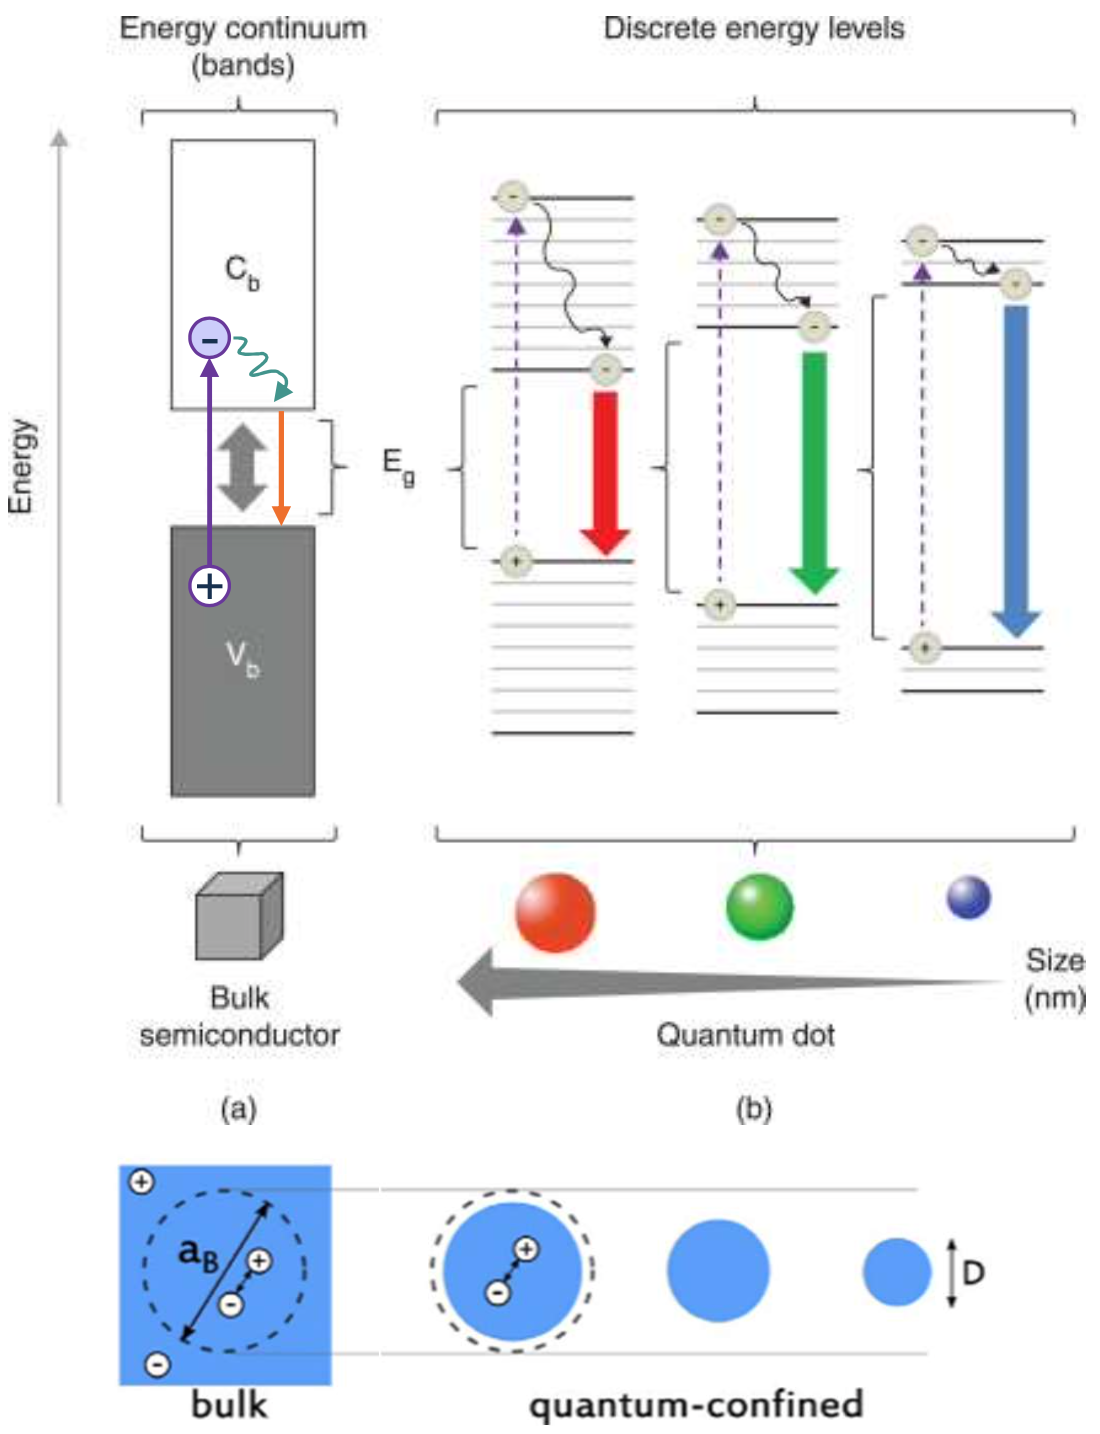
\includegraphics[width=0.4\linewidth]{QDotsConfinement.png}
        \caption{Quantum confinement effects in QDots.}
        \label{fig:QDotsConfinement}
    \end{figure}
    \begin{itemize}
        \item Nanomaterials: Size-dependent optical properties.
        \item The color changes from blue to red as the size of \ce{CdSe} nanodots grows from \SI{2}{\nano\meter} to \SI{8}{\nano\meter}.
        \item Why?
        \begin{itemize}
            \item In a bulk semiconductor, excitation creates an \textbf{exciton}.
            \item Excited electron and hole can diffuse.
            \item Dissipation of heat to lattice (via \textbf{phonons}).
            \item Emission of light at the bandgap $E_g$.
            \item The electron and hole attract coulombically, but there is a length scale in bulk; this is why size affects color.
        \end{itemize}
        \item Confinement: We confine the exciton to tiny sphere (like the particle in a box), but then only certain energy levels (corresponding to colors based on size) can be taken on.
        \item The Coulomb potential leads to hydrogen-like energies and wavefunctions.
    \end{itemize}
    \item \textbf{Exciton}: An electron-hole pair.
\end{itemize}



\section{Lab 5: ECHEM}
\begin{itemize}
    \item \marginnote{2/16:}\textbf{Hydrogen evolution reaction}: The synthesis of non-carbon-containing fuel (\ce{H2}) from protons (water or hydronium) and electrons. \emph{Also known as} \textbf{HER}. \emph{Given by}
    \begin{equation*}
        \ce{2H+ + 2e^- <=> H2}
    \end{equation*}
    \item Developing a rate law for the HER allows us to extract molecular-level insight into the chemistry of the catalyst active site.
    \item Thus, the goal of this lab is to: Develop a rate law for the HER consistent with experimental observations using physical electrochemistry techniques, and use it to further optimize key binding energetics of relevant intermediates.
    \item \textbf{Water-splitting}: The following reaction. \emph{Given by}
    \begin{equation*}
        \ce{2H2O <=> 2H2 + O2}
    \end{equation*}
    \begin{itemize}
        \item Stores \SI{1.23}{\volt} energy in chemical fuels.
    \end{itemize}
    \item Water-splitting electrochemical half-reactions.
    \begin{align*}
        \ce{2H+ + 2e^-} &\ce{<=>} \ce{H2}&
        \ce{2H2O} &\ce{<=>} \ce{4H+ + 4e^- + O2}
    \end{align*}
    \begin{itemize}
        \item The left one is the HER!
    \end{itemize}
    \item \textbf{Reduction potential}: The tendency of a chemical species to be reduced by gaining an electron. \emph{Also known as} \textbf{thermodynamic potential}.
    \item \textbf{Standard Hydrogen Electrode}: The reduction potential of the HER in \SI{1}{\molar} acid conditions and at one atmosphere of \ce{H2}. \emph{Also known as} \textbf{SHE}. \emph{Given by}
    \begin{equation*}
        E_{\ce{H+}/\ce{H2}} = 0.00
    \end{equation*}
    \item \textbf{Nernst equation}: The relationship between the standard reduction potential and the reduction potential at nonstandard conditions. \emph{Given by}
    \begin{equation*}
        E = E^\circ-\frac{RT}{nF}\ln Q
    \end{equation*}
    \item \textbf{Nerstian} (response): A response in line with the Nernst equation.
    \item The reduction potential for any electrochemical reaction involving the consumption or production of protons will exhibit a \textbf{Nerstian} response due to changes in $\pH$ conditions.
    \begin{itemize}
        \item It follows that
        \begin{equation*}
            E_{\ce{H+}/\ce{H2}} = E_{\ce{H+}/\ce{H2}}^\circ-\frac{RT}{nF}\ln(\frac{P_{\ce{H2}}}{[\ce{H+}]^2})
        \end{equation*}
        \item Under our conditions of \SI{25}{\celsius} and unit $P_{\ce{H2}}$, we obtain the following equation.
        \begin{align*}
            E_{\ce{H+}/\ce{H2}} &= E_\text{SHE}-\frac{\left( \SI[per-mode=fraction]{8.31}{\joule\per\mole\per\kelvin} \right)\left( \SI{298}{\kelvin} \right)}{(2)\left( \SI{96485}{\coulomb\per\mole} \right)}\ln(\frac{1}{[\ce{H+}]^2})\\
            &= E_\text{SHE}-\frac{\left( \SI[per-mode=fraction]{8.31}{\joule\per\mole\per\kelvin} \right)\left( \SI{298}{\kelvin} \right)}{(2)\left( \SI{96485}{\coulomb\per\mole} \right)}\cdot\frac{\log_{10}([\ce{H+}]^{-2})}{\log_{10}(\e)}\\
            &= E_\text{SHE}-\frac{\left( \SI[per-mode=fraction]{8.31}{\joule\per\mole\per\kelvin} \right)\left( \SI{298}{\kelvin} \right)}{(2)\left( \SI{96485}{\coulomb\per\mole} \right)(\log_{10}(\e))}\cdot 2\cdot -\log_{10}([\ce{H+}])\\
            &= E_\text{SHE}-\frac{\left( \SI[per-mode=fraction]{8.31}{\joule\per\mole\per\kelvin} \right)\left( \SI{298}{\kelvin} \right)}{\left( \SI{96485}{\coulomb\per\mole} \right)(\log_{10}(\e))}\cdot\pH\\
            &\approx E_\text{SHE}-0.059\cdot\pH
        \end{align*}
    \end{itemize}
    \item To account for the affect of $\pH$, we often reference the potential for the HER against the \textbf{Reversible Hydrogen Electrode} instead of the SHE.
    \item \textbf{Reversible hydrogen electrode}: The electrode with potential defined as follows. \emph{Also known as} \textbf{RHE}. \emph{Given by}
    \begin{equation*}
        E_\text{RHE} = E_\text{SHE}-0.059\cdot\pH
    \end{equation*}
    \item \textbf{Water oxidation reaction}: The other half-reaction involved in water-splitting. \emph{Given by}
    \begin{equation*}
        \ce{2H2O <=> 4H+ + 4e^- + O2}
    \end{equation*}
    \item The reduction potential for the water oxidation reaction is \SI{1.23}{\volt} vs. SHE.
    \begin{itemize}
        \item In other words, at potentials below \SI{1.23}{\volt}, water will be favored, and vice versa at potentials above \SI{1.23}{\volt}.
        \item Also Nerstian.
    \end{itemize}
    \item \textbf{Pourbaix diagram}: A diagram depicting the thermodynamic scaling of reduction potential as a function of $\pH$.
    \begin{itemize}
        \item Alternative definition: A phase diagram of sorts that indicates the thermodynamically stable phase of an electrochemical system.
    \end{itemize}
    \item Example: Pourbaix diagram for \ce{H2O}.
    \begin{figure}[h!]
        \centering
        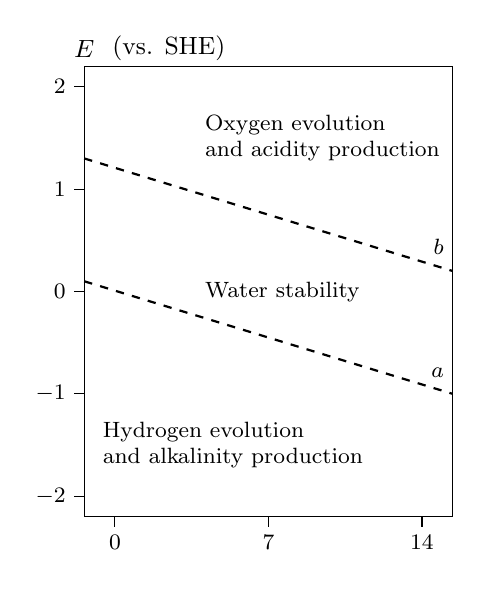
\begin{tikzpicture}[scale=1.3]
            \small
            \draw (-1.8,-2.2) -- node[below=6mm]{$\pH$} (1.8,-2.2) -- (1.8,2.2) -- (-1.8,2.2) node[above,label={right:(vs. SHE)}]{$E$} -- cycle;
    
            \footnotesize
            \draw
                (-1.5,-2.2) -- ++(0,-0.1) node[below]{0}
                (0,-2.2)    -- ++(0,-0.1) node[below]{7}
                (1.5,-2.2)  -- ++(0,-0.1) node[below]{14}
            ;
            \draw
                (-1.8,2)  -- ++(-0.1,0) node[left]{$2$}
                (-1.8,1)  -- ++(-0.1,0) node[left]{$1$}
                (-1.8,0)  -- ++(-0.1,0) node[left]{$0$}
                (-1.8,-1) -- ++(-0.1,0) node[left]{$-1$}
                (-1.8,-2) -- ++(-0.1,0) node[left]{$-2$}
            ;
    
            \draw [dashed,thick]
                (-1.8,1.3) -- ++(3.6,-1.1) node[above left,yshift=1mm]{$b$}
                (-1.8,0.1) -- ++(3.6,-1.1) node[above left,yshift=1mm]{$a$}
            ;
    
            \node [anchor=west,align=left] at (-1.7,-1.5) {Hydrogen evolution\\and alkalinity production};
            \node [anchor=west]            at (-0.7,0)    {Water stability};
            \node [anchor=west,align=left] at (-0.7,1.5)  {Oxygen evolution\\and acidity production};
        \end{tikzpicture}
        \caption{Pourbaix diagram for \ce{H2O}.}
        \label{fig:PourbaixH2O}
    \end{figure}
    \begin{itemize}
        \item Line $a$ corresponds to hydrogen evolution. It has $y$-intercept $(0,0)$.
        \item Line $b$ corresponds to oxygen reduction. It has $y$-intercept $(0,1.23)$.
        \item Both lines have a slope of $-\SI{0.059}{\volt\per pH}$.
    \end{itemize}
    \item Note that for practical reasons (side reactions, voltage lost as heat, etc.), application of a substantially higher voltage is necessary for the HER to proceed at a practical rate.
    \item \textbf{Overpotential}: The extra potential needed to overcome the kinetic barriers inherent to the half reactions.
    \item "The central challenge for chemistry is to develop catalysts to bring the operational potential as close to the thermodynamic potential as possible."
    \item Choosing catalysts.
    \begin{itemize}
        \item The catalytic activity of solid electrodes toward the HER correlates with their surface metal hydride bond strength.
        \item The correlation forms a volcano plot: When the metal hydride bond is too weak, there is not enough driving force to initiate the reaction; when it is too strong, the reaction is inhibited.
        \item Takeaway: \ce{Pt} is best (by this \textbf{descriptor}).
        \item Other concerns include oxidation/corrosion of the metal surface.
    \end{itemize}
    \item \textbf{Descriptor}: A (possibly incomplete) measure of something.
    \item Three materials we'll be working with: \ce{TiO_x}, \ce{SnO_x}, and \ce{PtO_x}.
    \item \textbf{Working electrode}: The electrode material of interest. \emph{Also known as} \textbf{w.e.}
    \item \textbf{Reference electrode}: The electrode of known potential. \emph{Also known as} \textbf{r.e.}
    \item Such a \textbf{two-electrode cell} can determine the $i$-$E$ curve.
    \item With more highly resistive solutions, a \textbf{three-electrode cell} is preferable.
    \begin{figure}[h!]
        \centering
        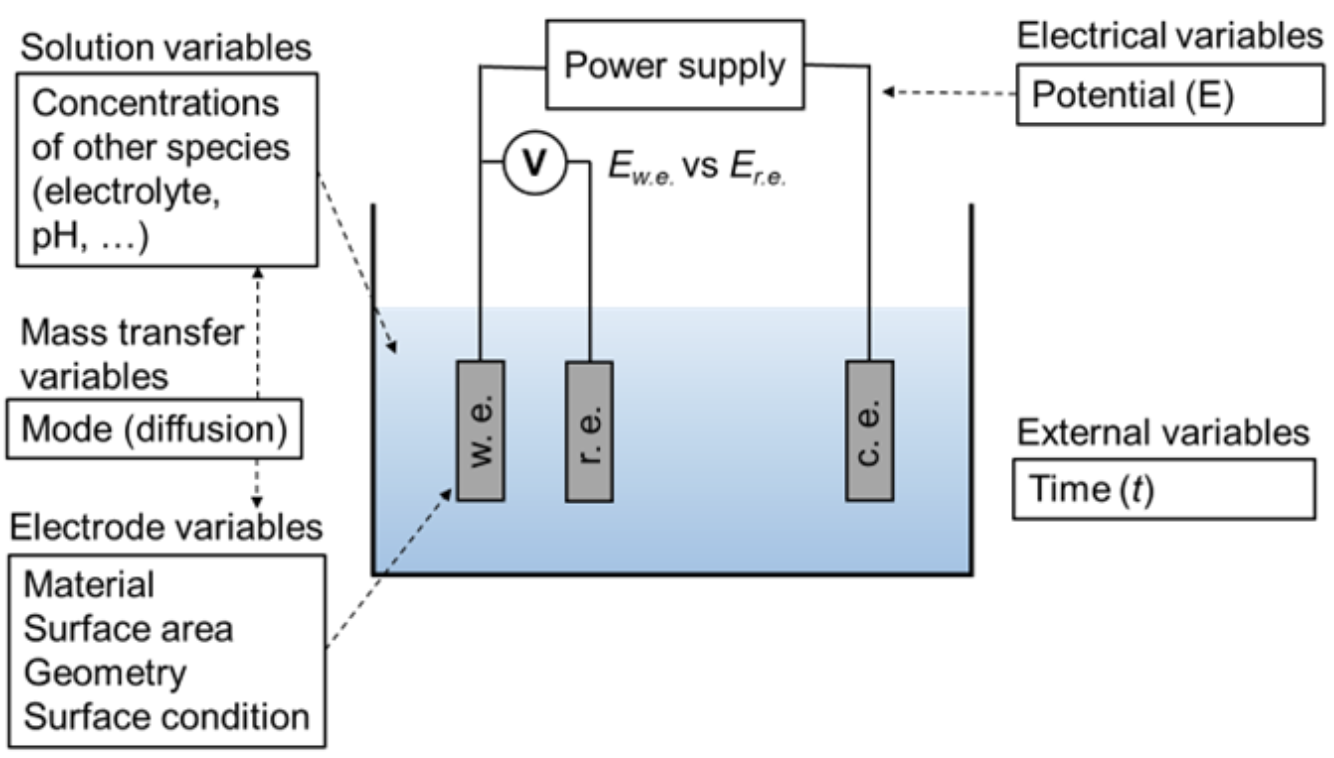
\includegraphics[width=0.5\linewidth]{3electrodeCell.png}
        \caption{Schematic three-electrode cell with variables affecting the rate of reaction.}
        \label{fig:3electrodeCell}
    \end{figure}
    \begin{itemize}
        \item Such a setup involves an additional \textbf{counter electrode}, or \textbf{c.e.}
        \item The material of the c.e. does not matter since it won't affect the behavior of the w.e.
    \end{itemize}
    \item Steps on the first day.
    \begin{itemize}
        \item For each electrocatalyst, we'll take a CV first to figure out where the overpotential is.
        \item We'll then identify points along the foot of the wave at which to collect \textbf{chronoamperograms}.
    \end{itemize}
    \item CV.
    \begin{figure}[h!]
        \centering
        \begin{subfigure}[b]{0.45\linewidth}
            \centering
            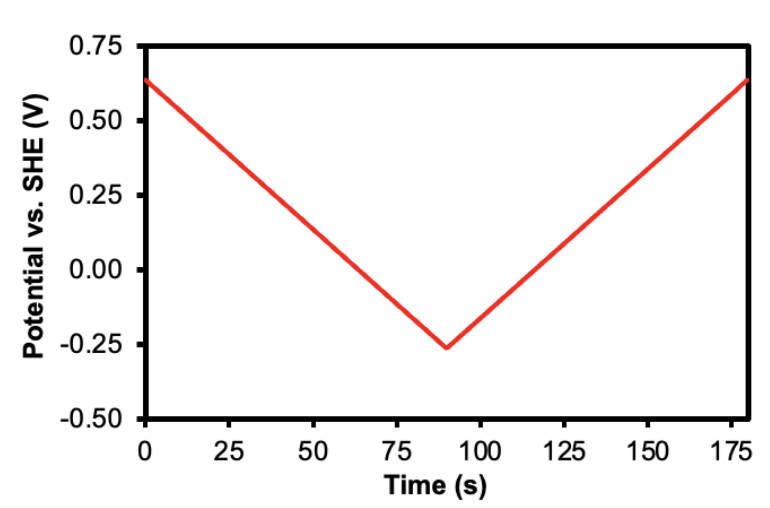
\includegraphics[width=0.9\linewidth]{CVa.png}
            \caption{Sweeping potential.}
            \label{fig:CVa}
        \end{subfigure}
        \begin{subfigure}[b]{0.45\linewidth}
            \centering
            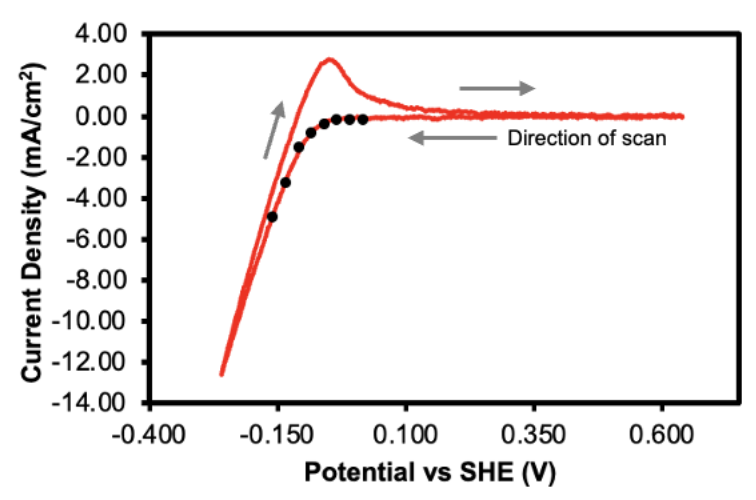
\includegraphics[width=0.9\linewidth]{CVb.png}
            \caption{Cyclic voltammagram.}
            \label{fig:CVb}
        \end{subfigure}
        \caption{Cyclic voltammetry.}
        \label{fig:CV}
    \end{figure}
    \begin{itemize}
        \item Figure \ref{fig:CVa} shows the potentials we sweep over, first negative and then positive, as time progresses. Notice that this change in potential is mirrored by the grey arrows in Figure \ref{fig:CVb}.
        \item Figure \ref{fig:CVb} shows the cyclic voltammagram. The black points lie along the foot of the wave and are where we want to collect CA data. They correspond to overpotentials that induce catalysis.
    \end{itemize}
    \item \textbf{Chronoamperometry}: The measure of the current (or current density, when normalized to the surface area of the working electrode) that flows as a function of time when a working electrode is poised at a specific potential. \emph{Also known as} \textbf{CA}.
    \begin{figure}[h!]
        \centering
        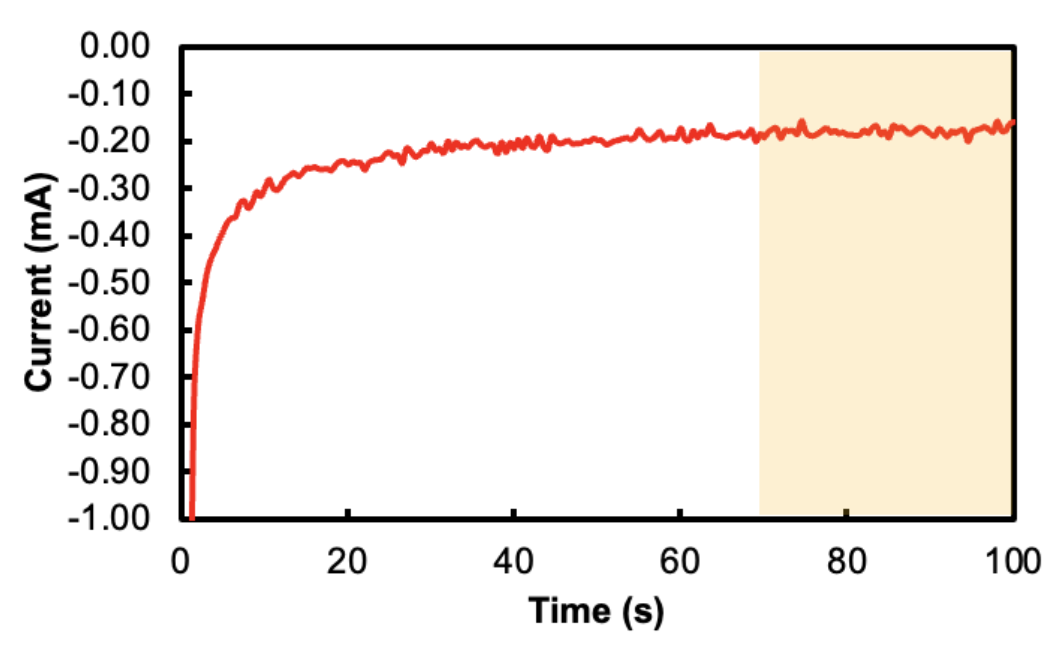
\includegraphics[width=0.5\linewidth]{CA.png}
        \caption{Chronoamperometry.}
        \label{fig:CA}
    \end{figure}
    \begin{itemize}
        \item We have an initially high charging current which decays exponentially with time, after which \textbf{Faradiac current} flows.
    \end{itemize}
    \item \textbf{Faradaic current}: The current attributed to electron transfer events.
    \begin{itemize}
        \item In this case, this is the current attributed to \ce{H2} evolution.
    \end{itemize}
    \item Creating a Tafel plot.
    \begin{itemize}
        \item To extract kinetic and thermodynamic parameters and investigate the mechanism, we'll construct a Tafel plot for each electrode under each $\pH$ fo interest.
        \item Average the current density that flows over the last 30 seconds of the 100 second CA experiment (the yellow region in Figure \ref{fig:CA}).
        \item Plot the log of the negative of this value against the overpotential at which it was collected.
    \end{itemize}
    \item We will be using a \ce{Hg/HgSO4} (saturated \ce{K2SO4}) electrode, which has a potential of \SI{0.650}{\volt} vs. SHE.
    \begin{itemize}
        \item Thus, I should (where asked) convert any measured potentials to SHE via
        \begin{equation*}
            E_\text{SHE}(\si{\volt}) = E_{\ce{Hg/Hg2SO4}}(\si{\volt})+\SI{0.650}{\volt}
        \end{equation*}
        and then to RHE via its definition.
    \end{itemize}
    \item \textbf{Overpotential} (for a reductive process): The quantity defined as follows. \emph{Denoted by} $\bm{\eta}$. \emph{Given by}
    \begin{equation*}
        \eta(\si{\volt}) = E_{\ce{2H+/H2}}-E_\text{app}
    \end{equation*}
    \item Steps on the second day.
    \begin{itemize}
        \item Measure the $\pH$ dependence of the HER on \ce{Pt} by collecting the same set of CVs and CAs over a range of $\pH$ values.
    \end{itemize}
    \item Mechanisms of HER.
    \begin{figure}[H]
        \centering
        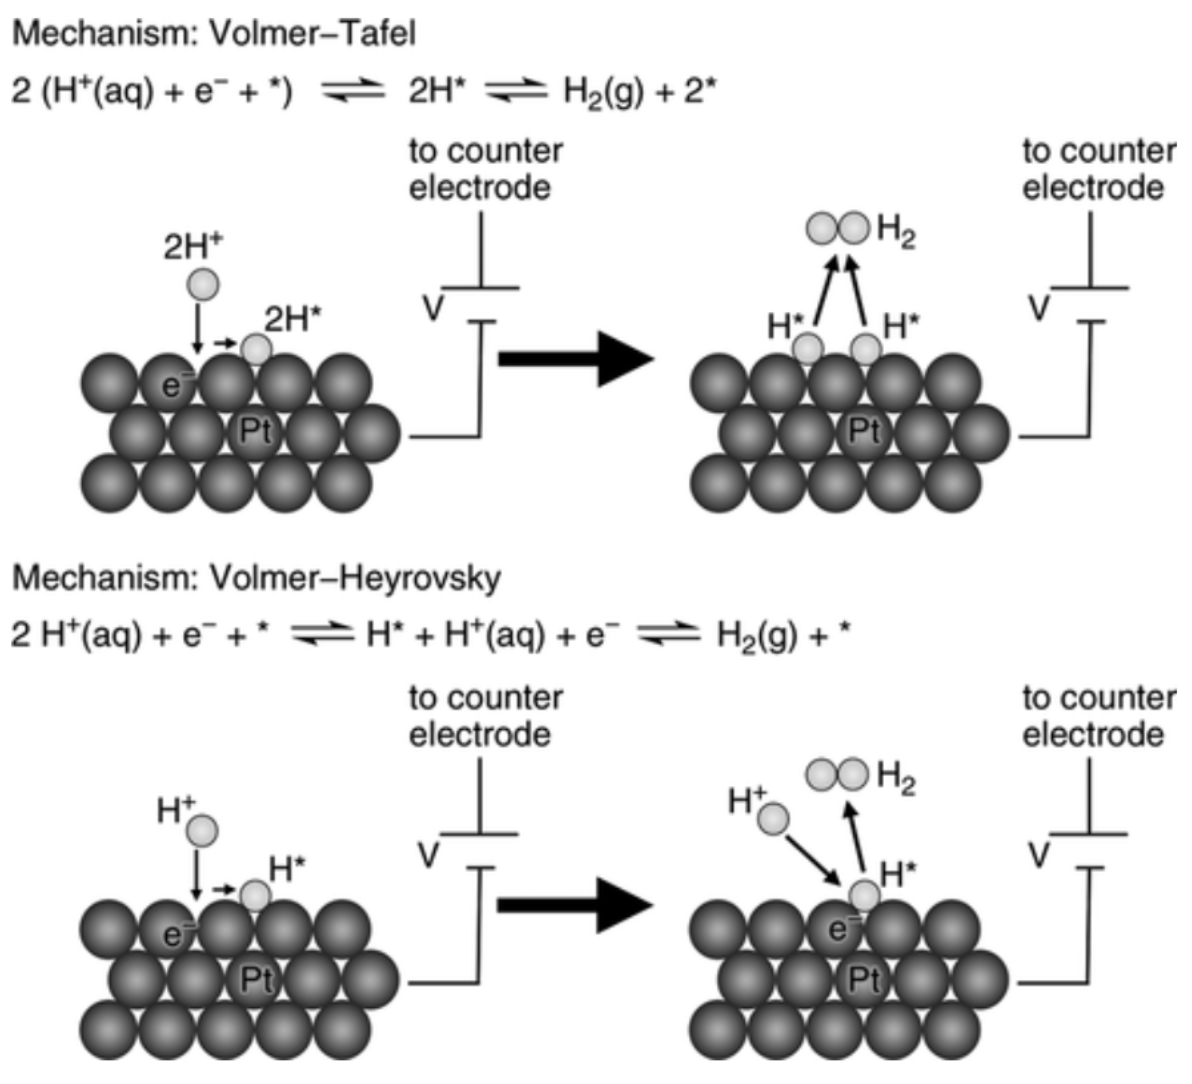
\includegraphics[width=0.5\linewidth]{HERmechanism.png}
        \caption{HER mechanisms.}
        \label{fig:HERmechanism}
    \end{figure}
    \item \textbf{Volmer-Tafel} (mechanism of HER): Both proton and electron are used to make a surface-bound \ce{H}, and then two surface bound hydrogen atoms recombine to form \ce{H2}.
    \item \textbf{Volmer-Heyrovsky} (mechanism of HER): Only one pair of proton and electron forms a surface-bound hydrogen, which is then protonated and reduced in a single step to form \ce{H2}.
    \item Distinguishing between the two mechanisms.
    \begin{figure}[h!]
        \centering
        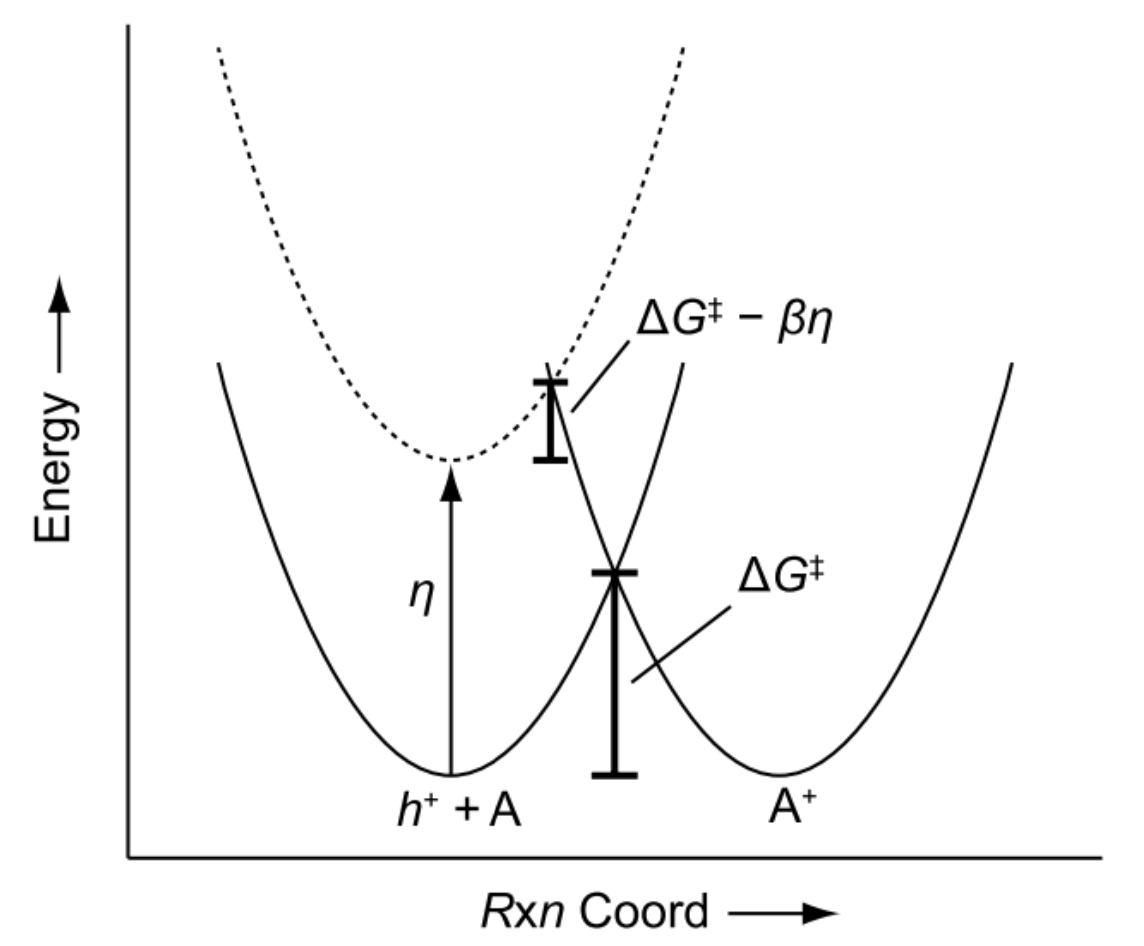
\includegraphics[width=0.4\linewidth]{EChemRCD.png}
        \caption{Reaction coordinate diagram.}
        \label{fig:EChemRCD}
    \end{figure}
    \begin{itemize}
        \item Quantities in Figure \ref{fig:EChemRCD}.
        \begin{itemize}
            \item \ce{h+} is a hole with chemical potential equal to the Fermi level of the poised electrode.
            \item $\Delta G^\ddagger$ is the activation battier.
            \item $\eta$ is the overpotential.
            \item $\beta$ is the \textbf{symmetry factor}.
            \item The reaction under study is single-electron oxidation of \ce{A}.
        \end{itemize}
        \item Assume that the total current we measure goes toward the HER.
        \begin{itemize}
            \item Formally, we say that the Faradaic efficiency is 100\%.
            \item This assumption is experimentally supported
        \end{itemize}
        \item We monitor and control reaction rate via
        \begin{equation*}
            j = nFv
        \end{equation*}
        where $j$ is current density, $n$ is the equivalents of electrons, $F$ is Faraday's constants, and $v$ is the velocity of the reaction (\si{mol.e^-\per\second}).
        \item We tune the potentials in Figure \ref{fig:EChemRCD} by adjusting the potential (which directly alters the energy of the electron).
        \item By the \textbf{Eyring equation}, there is an exponential relationship between activation barrier and reaction rate. In this case, this means that tuning the overpotential will lead to an exponential increase in activation-controlled current density, i.e.,
        \begin{equation*}
            j = j_0\e[\beta\eta F/RT]
        \end{equation*}
        \item Rearranging the above and taking the base 10 logarithm yields
        \begin{equation*}
            \text{Tafel slope} = \frac{2.3RT}{\beta F}
        \end{equation*}
        \item We take $\beta=0.5$ for processes such as this one with high \textbf{reorganizational energy}.
        \item Derivation that Volmer-Tafel has a slope of 30 mV/log j and Volmer Heyrovsky has a slope of 120 mV/log j.
    \end{itemize}
    \item \textbf{Symmetry factor}: The fraction of the overpotential that goes toward lowering the activation of the electron transfer process. \emph{Denoted by} $\bm{\beta}$.
    \item \textbf{Reorganizational energy}: The energy required to rearrange the solvent after a redox reaction.
\end{itemize}


\subsection*{In Lab}
\subsubsection*{Day 1}
\begin{itemize}
    \item \ce{Pt}.
    \item Open circuit potential: \SI{234.1}{\milli\volt}.
    \item Ru: \SI{51.888}{\ohm}.
    \item CV plot: Scanning right to left, we eventually induce the HER. Then on the way back, we oxidize leftover hydrides off of the catalyst surface.
    \begin{itemize}
        \item This comes from previous literature; we can't derive that just from the CV.
    \end{itemize}
    \item \ce{Ti} electrode area: $\SI{9}{\milli\meter}\times\SI{7}{\milli\meter}$.
    \item \ce{Sn} electrode area: $\SI{8}{\milli\meter}\times\SI{6}{\milli\meter}$.
    \item \ce{Pt} electrode area: diameter $\SI{2}{\milli\meter}$.
    \item \ce{Sn}.
    \item OCP: $-\SI{928.2}{\milli\volt}$.
    \item Ru: \SI{9.508}{\ohm}.
    \item We have an oxide forming in solution; this means that the electrolyte will need to be switched out before our next run.
    \item Huge corrosion.
    \item \ce{Ti}.
    \item OCP: $-\SI{227.5}{\milli\volt}$.
    \item Ru: \SI{2.11}{\ohm}.
\end{itemize}




\end{document}